The following architectural styles and patterns have been used:

\subsubsection{Client and server}
The client-server model is used at different levels in the \emph{PowerEnJoy} system design:
\begin{itemize}
\item the mobile and the on-board applications are clients with respect to the Application Server that receives and elaborate requests.
\item the user's browser communicates with the Web Server. The first one is the client while the latter is in charge of providing a service, that is the requested web page.
\item the Web Server, as a client, communicates with the Application Server in order to process user's requests.
\item the Application Server, in the role of the client, queries the Database that is responsible for getting results.
\end{itemize}

\subsubsection{Multitier architecture}
The client-server multilayered architecture allows to physically separate presentation, application processing and data management operations.

Moreover, despite the fact the separation of the Web Server from the Application Server increments the number of tiers in the system, it brings a huge improvement in service availability because in case of Web Server failure, the system remains still accessible from the mobile application.

\subsubsection{Thin client}
The think client approach has been used with respect to the interaction among user's machines and the system itself.

All the main logic is implemented by the Application Server that has a decent computing power and can manage concurrency issues in an efficient way. On the other hand, the mobile application and the user's browser are in charge of presentation only and they do not involve decision logic.

This choice is also reasonable because allows users to take advantage of the service via devices with limited computing power and makes software updates easier.

\subsubsection{Thick client}
The on-board application has been designed to involve a discrete amount of logic, but still requires a periodic connection to the central Application Server in order to work properly.

Its logic mainly deals with the control of the car systems, such as unlocking the doors, and gathering information from several sensors placed in the cabin. Furthermore the application has to detect different discount and additional charges situations, that affects the final charge the user has to pay, and communicates them to the Application Server.

\subsubsection{Model-View-Controller}
The web, the mobile and the on-board applications follow the Model-View-Controller software design pattern. The MVC allows to separate the application into three communicating and interconnected parts fulfilling the design principle of the separation of concerns.

%Siamo sicuri che non ci sia una distributed presentation per quanto riguarda la web application?

\begin{figure}[H]
\begin{center}
		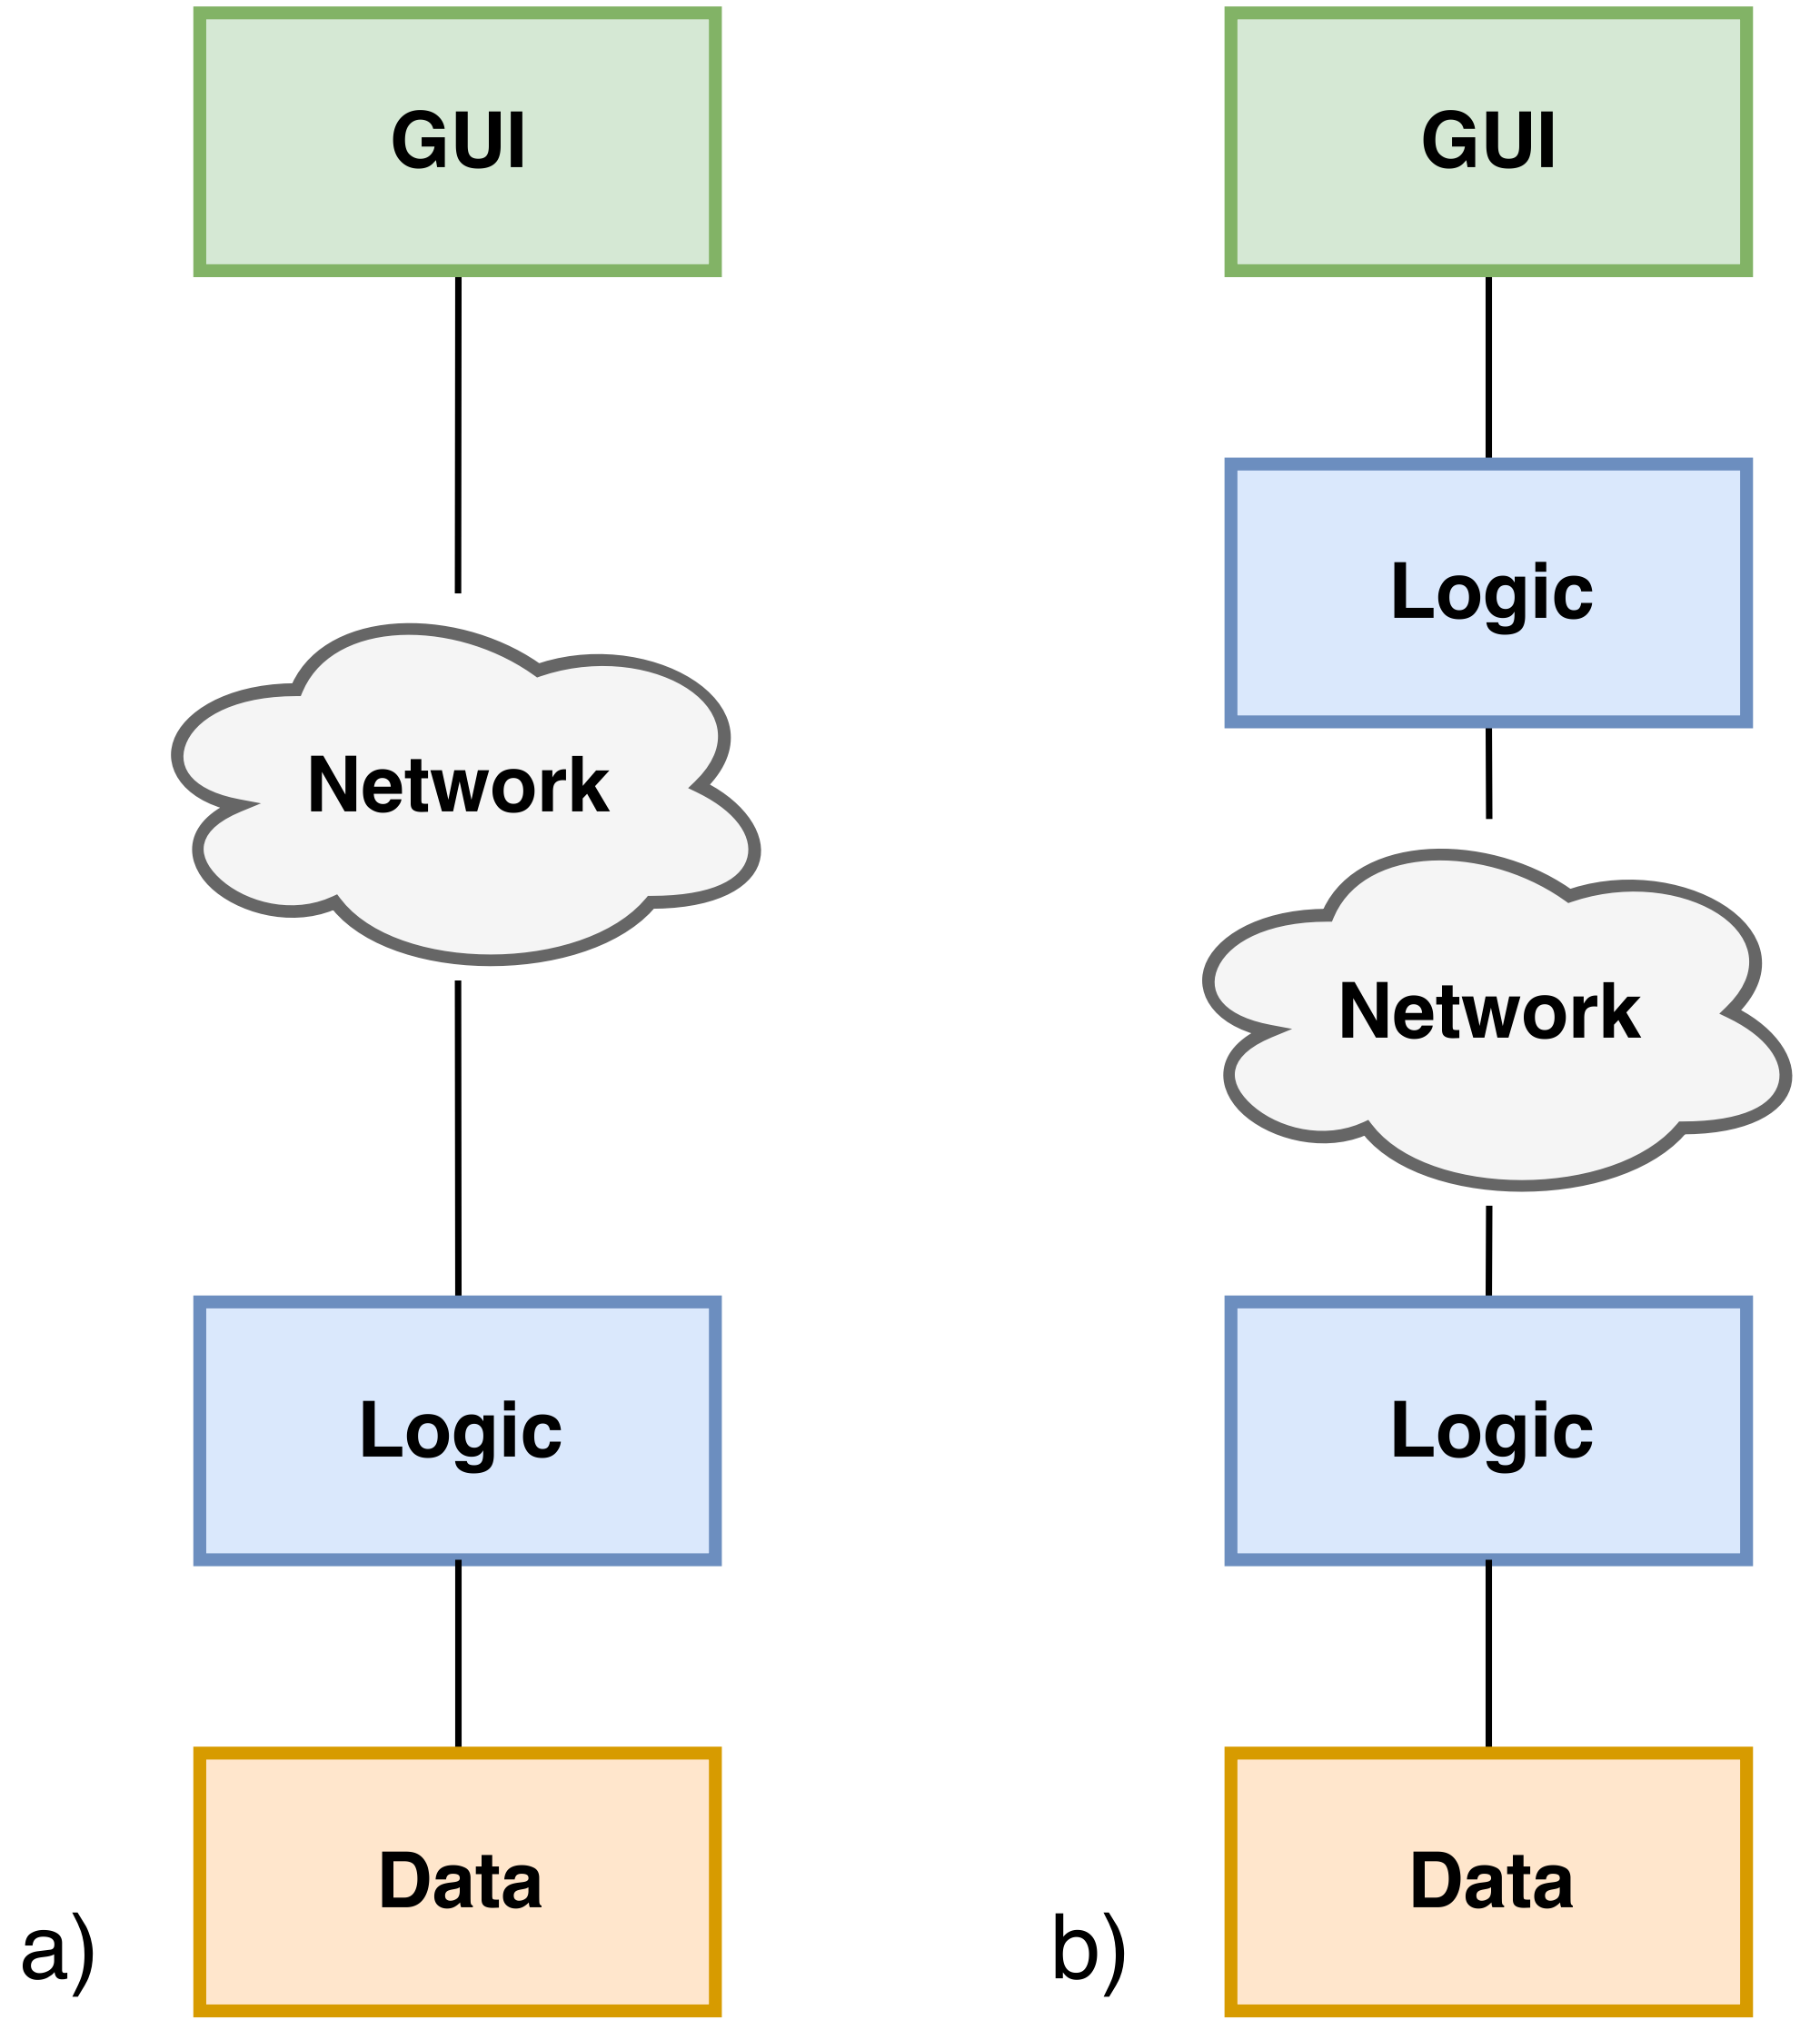
\includegraphics[width=0.4\textwidth]{./arch_design/diagrams/architectural_patterns.png}
		\caption{The remote presentation (a) and the distributed logic (b) architectural styles that inspired respectively the design of the mobile and the on-board application.}
		\label{er_dg}
\end{center}
\end{figure}